\chapter{Lógica modal clásica}
\label{cap:logclasica}

Usualmente, existen situaciones donde necesitamos como herramienta de modelado una lógica que tenga buenas propiedades computacionales. En estos casos, la lógica de primer orden ($\mathsf{LPO}$)~\cite{enderton72} no es la mejor alternativa. En particular, las tareas de inferencia para $\mathsf{LPO}$ no son tratables computacionalmente. Por ejemplo, el problema de determinar si una fórmula $\varphi$ de $\mathsf{LPO}$ es satisfacible, es indecidible \cite{chur:note36,turi:comp37,berg:unde66}, mientras que \emph{model checking} (es decir, dado un modelo $\M$ y una fórmula $\varphi$, determinar si $\M$ satisface $\varphi$) es $\sf{PSPACE}$-completo \cite{Stockmeyer74,chan:opti77,Vardi82}. Por este motivo, es natural buscar nuevos lenguajes con mejores propiedades computacionales. Las lógicas modales~\cite{blackburn01,blackmodal06} se encuentran dentro de esta familia de lógicas: son lógicas diseñadas para hablar de estructuras relacionales lo cual permite su utilización en diversos campos: ling\"uística, verificación de software, teoría de juegos, etc. Es por este motivo que las lógicas modales resultan una elección tan recurrente en ciencias de la computación: en general, poseen un buen balance entre expresividad y comportamiento computacional.

En este trabajo nos dedicaremos al estudio de lógicas modales intuicionistas. En este capítulo, comenzaremos por introducir las nociones básicas de la lógica modal clásica: su sintaxis, su semántica, y una discusión sobre su teoría de prueba, para luego trabajar sobre el caso intuicionista en los capítulos siguientes.

\section{Sintaxis y semántica}
El lenguaje de la lógica modal básica se obtiene extendiendo lógica proposicional clásica con los conectivos modales $\square$ y $\Diamond$, los cuales históricamente representan \textit{necesidad} y \textit{posibilidad} respectivamente. 

\dfn Sea $\mathsf{PROP}$ un conjunto infinito contable de proposiciones atómicas, las fórmulas modales se construyen a partir de la siguiente gramática:
\begin{center}
	 $A ::=  a$ $| $ $\vls-a$ $ | $  $\top$ $|$ $\bot $ $|$ $\vls(A.A)$ $|$ $\vls[A.A]$ $|$  $\square A$ $|$ $\Diamond A$,
\end{center} 
\noindent donde $a \in A$ y $\vls-a$ es su negación.


Siempre asumimos que las fórmulas están en \textit{negation normal form}, esto es, la negación está restringida a los átomos. Cuando escribimos $\neg A$, nos referimos al resultado de computar la \emph{negation normal form}, utilizando las siguientes equivalencias: $\neg a \equiv \vls-a$, $\neg \vls-a \equiv a$, $\neg \neg A $ $\equiv$ $A$, $\neg (\vls(A.B))\equiv \vls[\neg A. \neg B]$ y $\neg \square A \equiv \Diamond \neg A$, donde $\equiv$ denota equivalencia. La implicación material puede ser definida a partir de este conjunto de conectivos como: $A \vljm B \coloneqq \vls[\neg A. B]$. $\top$ and $\bot$ son las constantes usuales denotando verdadero y falso respectivamente.

Como dijimos anteriormente, las fórmulas de lógica modal se interpretan sobre estructuras relacionales. Por razones históricas, dichas estructuras se conocen como modelos de Kripke \cite{kripke1959}. La semántica en términos de estos modelos se conoce como \emph{semántica de Kripke} o por la interpretación original de los operadores modales, como \emph{semántica de mundos posibles}. Intuitivamente, un modelo es un grafo dirigido con etiquetas en los nodos, y las fórmulas modales permiten expresar propiedades de estos grafos. A la estructura relacional, sin considerar las etiquetas en los nodos, se la conoce como \emph{frame}. A continuación introducimos formalmente la definición de frame y de modelo de Kripke.


\dfn(Frame) Un \textit{frame} es un par $\langle W, R\rangle$ donde $W$ es un conjunto no vacío de mundos posibles y $R$ es una relación binaria (mejor conocida como \textit{relación de accesibilidad}) tal que $R \subseteq W\times W$.

Las lógicas modales permiten describir axiomáticamente propiedades estructurales de un modelo, es decir propiedades del frame. Ejemplos de esto pueden ser reflexividad, transitividad, o simetría de la relación de accesibilidad. 

Agregando valuaciones a los mundos, obtenemos los modelos de Kripke:

\dfn(Modelos de Kripke) Un \textit{modelo} $\M$ es una tupla $\langle W, R, V \rangle$, donde $\langle W, R \rangle$ es un frame, y $V : W \rightarrow 2^{\mathsf{PROP}}$ es una función de valuación, que asigna a cada mundo $w$ un conjunto de variables proposicionales que se hacen verdaderas en $w$. Sea $w \in W$, llamamos a $\M, w$ un \emph{pointed model}.

La Figura~\ref{fig:kmodel}  muestra un ejemplo de un modelo de Kripke. Podemos observar que el modelo $\M$ es un grafo con 3 elementos, $\cset{w,v,u}$. 
$w$ está etiquetado con $p$, $u$ con $p$ y $q$, y $v$ no posee etiqueta.
Formalmente, $\M{=}\tup{W,R,V}$, donde $W=\cset{w,v,u}$, $R=\cset{(w,v),(w,u),(v,v),\linebreak (v,u),(u,v)}$, y $V(w){=}\cset{p},V(u)=\cset{p, q}$. 

\begin{figure}[h]
	\begin{center}
		\begin{tikzpicture}[>=latex]
		\node (a0) at (-1,0)   [shape=circle,draw,fill, inner sep=1pt,label=above left:$w$,label=below left:$\cset{p}$] {} ;
		\node (a1) at (1,1)  [shape=circle,draw,fill, inner sep=1pt, label=right:$v$] {} ;
		\node (a2) at (1,-1)  [shape=circle,draw,fill, inner sep=1pt, label=right:$u$,label=below:$\cset{p,q}$] {} ;
		\draw [ar,->] (a0) edge [bend left] (a1);
		\draw [ar,->] (a0) edge [bend right] (a2);
		\path [ar,->] (a1) edge [loop] (b0);
		\draw [ar,->] (a1) edge [bend left] (a2);
		\draw [ar,->] (a2) edge [bend left] (a1);
		\node (a3) at (-1.5,-.9)  [] {$\M$} ;
		\end{tikzpicture}
	\end{center}
	\caption{Ejemplo de un modelo de Kripke.}
	\label{fig:kmodel}
\end{figure}


Una proposición expresada por una fórmula que involucra solo los conectivos lógicos de la lógica proposicional se determina localmente sobre un mundo en particular y es independiente del estado de otros \emph{mundos}. Por otra parte, una proposición expresada por una fórmula que involucra las modalidades depende fundamentalmente del estado de otros \emph{mundos}. En un mundo \emph{w}, la fórmula $\Diamond A$ expresa la proposición de que $A$ es cierta en algún mundo $v$ considerado posible desde el punto de vista de $w$ (técnicamente, la definición de que $v$ es posible de acuerdo con $w$ será modelada por la relación de accesibilidad del modelo). Dualmente, la fórmula $\square A$ expresa la proposición (en $w$) de que $A$ es verdadera en todos los mundos $v$ considerados posibles por $w$. De este modo, el significado de las modalidades $\square$ y $\Diamond$ recibe una lectura basada en la noción primitiva de verdad relativa, es decir, verdad en un mundo.


Los operadores de la lógica modal básica describen propiedades \emph{locales} de los modelos, lo que significa que las fórmulas son evaluadas en algún punto específico. Para eso usamos \emph{pointed models}.

\dfn Sea $\M = \langle W, R, V \rangle $ un modelo, $w \in W$ y $A$ una fórmula, decimos que $\M, w $ satisface $A$ (denotado $\M, w \Vdash A$) si: %\male{se ve feo así! no te parece?}
	$$
	\begin{array}{rcl}
	
 \M, w \Vdash a & \mbox{sii} & a \in V(w)\\
 
	\M, w \Vdash \vls-a& \mbox{sii} & a \not \in V(w)\\
	
	\M, w \Vdash A \vlan B & \mbox{sii} & \M, w \Vdash A\mbox{ y }\M, w \Vdash B \\
	
	\M, w \Vdash A \vlor B & \mbox{sii} & \M, w \Vdash A\mbox{ o }\M, w \Vdash B \\
	
	\M, w \Vdash \square A & \mbox{sii} & \mbox{para todo } v \in W \mbox{ tal que } wRv \mbox{ y } \M, v \Vdash A \\
	
	\M, w \Vdash \Diamond A & \mbox{sii} & \mbox{existe } v \in W \mbox{ tal que } wRv \mbox{ y } \M, v \Vdash A \\
\end{array}$$
%\hspace{9mm}	$\M, w \Vdash a$ si y sólo si $a \in V(w)$

%\hspace{9mm}	$\M, w \Vdash \vls-a$ si y sólo si $a \not \in V(w)$

%\hspace{9mm}	$\M, w \Vdash \vls(A.B)$ si y sólo si $\M, w \Vdash A$ y $\M, w \Vdash B$

%\hspace{9mm} $\M, w \Vdash \vls[A.B]$ si y sólo si $\M, w \Vdash A$ o $\M, w \Vdash B$

%\hspace{9mm} $\M, w \Vdash \square A$ si y sólo si para todo $v \in W$ tal que $(w, v) \in $ R y $\M, v \Vdash A$

%\hspace{9mm} $\M, w \Vdash \Diamond A$ si y sólo si existe un $v \in W$ tal que $(w, v) \in R$ y $\M, v \Vdash A$

\vspace{1mm}

Una fórmula $A$ es satisfacible si existe un pointed model $\M, w$ tal que $\M,w \Vdash A$. Diremos que una fórmula $A$ es válida en un modelo (notación $\M \vDash A$) $\M$ si y sólo si en todos los estados $w \in W$ vale $\M, w \Vdash A$.



Notemos la correspondencia entre $\square$ y el cuantificador $\forall$, así como también la correspondencia entre el operador $\Diamond$ y el cuantificador $\exists$. En particular, podemos identificar a la lógica modal clásica como un fragmento de la lógica de primer orden clásica simplemente internalizando su semántica en $\mathsf{LPO}$.

Como se mencionó anteriormente, en este trabajo nos interesa estudiar los teoremas y sus demostraciones, en particular, de la lógica modal intuicionista. Para ello veremos las demostraciones como objetos formales. Existen diferentes tipos de sistemas de pruebas para un lenguaje lógico, cada uno con ciertas características particulares. Por ejemplo, los sistemas \emph{á la Hilbert} en general consisten de un conjunto de axiomas, y unas pocas reglas que permiten inferir teoremas a partir de axiomas. En contrapartida, en los sistemas \emph{á la Gentzen} predominan las reglas de inferencia por sobre los axiomas. A continuación presentaremos ambos tipos de sistemas para la lógica modal clásica.
% Podemos definir la satisfabilidad de una fórmula de la siguiente manera:

% \dfn(Satisfabilidad y Validez de una fórmula) Una formula $A$ se \emph{satisface} en un modelo $M$=$\langle W, R, V \rangle$ si existe  $w \in W$ tal que $\M, w \Vdash A$. Lo denotaremos con $\M, w\vDash A$. Diremos que una fórmula $A$ es \emph{válida} en un modelo $\M$ si para todo $w \in W$, $\M, w \vDash A$. Lo denotamos con $\M \vDash A$


%%%%%%%%%%%%%%%%%%%%%%%%%
\section{Axiomatizaciones \emph{á la Hilbert}}

Presentaremos a la lógica modal básica y su teoría como la llamada lógica modal $\K$. La misma se obtiene a partir de una axiomatización arbitraria de la lógica proposicional clásica, agregando los siguientes componentes:


\begin{itemize}
	\item la regla de \textit{necesitación:} si $A$ es un teorema de $\K$, entonces $\square A$ también lo es.
	\item el axioma de \textit{distributividad}, normalmente escrito de la siguiente forma:
		\begin{center}
		$\kaxiom$ $\colon$ $\square(A \vljm B) \vljm (\square A \vljm \square B)$.
		\end{center}
\end{itemize}

Es importante mencionar que lo que llamamos un axioma aquí es de hecho, como es estándar en las axiomatizaciones al estilo de Hilbert, un esquema de axiomas, para evitar una mención explícita de la regla de sustitución. Más concretamente, una derivación es una lista de fórmulas que son instancias de algunos esquemas de axiomas dados o deducciones de fórmulas anteriores combinadas usando una regla de inferencia. Además, como estamos aceptando el esquema del axioma $k$ en nuestro sistema base, todas las lógicas que consideramos pertenecen a la familia de las \emph{lógicas modales normales}. Se pueden obtener lógicas modales más fuertes agregando a $\K$ otros axiomas que contienen los conectivos modales. Una clase de axiomas modales que serán de nuestro interés han sido propuestos por Lemmon y Scott en \cite{lemmon1977}. Estos axiomas denominados \emph{de Scott-Lemmon} están definidos esquemáticamente por una 4-upla de números naturales $\langle h, i, j, k \rangle$ como:
\begin{center}
	$\mathsf{\mbox{g}_{hijk}} := \Diamond^{h} \square^{i} A \vljm \square^{j}  \Diamond^{k} A$,
\end{center}
donde $\square^{n}$ denota $n$ ocurrencias de $\square$ ($ \Diamond^{n}$ denota $n$ ocurrencias de $\Diamond$). Notemos que en el caso clásico $\mathsf{\mbox{g}_{hijk}}$ y $\mathsf{\mbox{g}_{jkhi}}$ son equivalentes por De Morgan.

Consideraremos también una subclase particular de estos axiomas llamados \emph{path Scott-Lemmon axioms} que corresponden al caso donde $i + k$ es exactamente igual a 1. Por ejemplo, obtenemos el siguiente axioma:

\begin{center}
		$\mathsf{\mbox{g}_{h1j0}} := \Diamond^{h} \square A \vljm \square^{j} A$
\end{center}

Algunas ocurrencias específicas del axioma de Scott-Lemmon se han estudiando con distintos nombres, como por ejemplo:
  
  $$
\begin{array}{rcl}
	\mathsf{\mbox{g}_{0001}} & \mbox{corresponde al axioma} & \taxiom := A \vljm \Diamond A \\
	
	\mathsf{\mbox{g}_{0011}} & \mbox{corresponde al axioma} & \baxiom := A \vljm \square \Diamond A \\
	
	\mathsf{\mbox{g}_{0101}} & \mbox{corresponde al axioma} & \daxiom := \square A \vljm \Diamond A \\
	
	\mathsf{\mbox{g}_{1002}} & \mbox{corresponde al axioma} & \fouraxiom := \Diamond A \vljm \Diamond \Diamond A \\
	
	\mathsf{\mbox{g}_{1011}} & \mbox{corresponde al axioma} & \fiveaxiom := \Diamond A \vljm \square \Diamond A \\
	
	\mathsf{\mbox{g}_{1111}} & \mbox{corresponde al axioma} & \twoaxiom := \Diamond \square A \vljm \square \Diamond A
\end{array}
$$

Podemos notar que $\taxiom$, $\baxiom$, $\fouraxiom$ y $\fiveaxiom$ son \emph{path Scott-Lemmon axioms}, pero $\daxiom$ y $\twoaxiom$ no lo son.

Seleccionando subconjuntos de estos axiomas nos permite \emph{a priori} definir treinta y dos lógicas modales. Sin embargo, algunas de ellas coinciden. Por ejemplo, los conjuntos $\{ \baxiom, \fouraxiom \}$ y $\{ \taxiom, \fiveaxiom\}$ ambos dan como resultado la lógica modal conocida como $\sfive$. Se obtienen quince lógicas modales distintas que se extienden entre $\K$ y $\sfive$ y se pueden representar en un cubo, como se muestra en la Figura \ref{fig:cubesfive}. Este cubo es conocido como el \emph{cubo $\sfive$}.

\begin{figure}[h]
	\begin{center}
	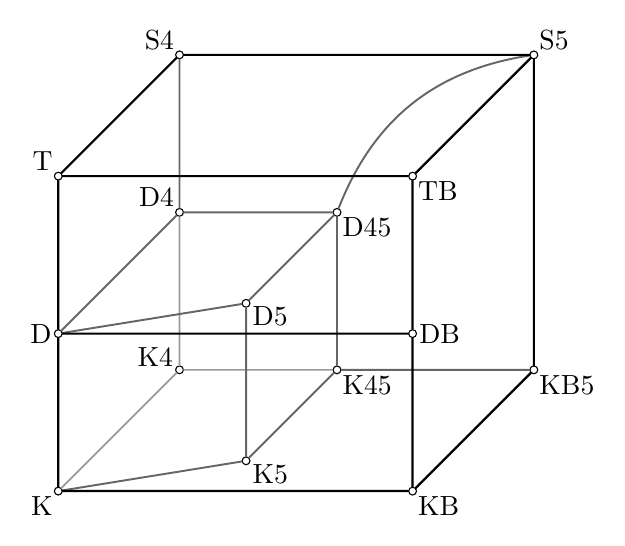
\begin{tikzpicture}
	[every node/.style={inner sep=1pt,outer sep=0},
	logic/.style={shape=circle,draw}]
	\def\xx{4.5}\def\hxx{2}\def\hhxx{2}
	\def\yy{4}\def\hyy{2}\def\hhyy{1}
	\def\zz{-4}\def\hzz{-2}\def\hhzz{-1}
	\node[logic,label=225:K]   (ik)   at (0, 0, 0)            {} ;
	\node[logic,label=-45:KB]  (ikb)  at (\xx, 0, 0)          {} ;
	\node[logic,label=-45:KB5] (ikb5) at (\xx, 0, \zz)        {} ;
	\node[logic,label=170:K4]  (ik4)  at (0, 0, \zz)          {} ;
	\node[logic,label=180:D]   (id)   at (0, \hyy, 0)         {} ;
	\node[logic,label=135:T]   (it)   at (0, \yy, 0)          {} ;
	\node[logic,label=135:S4]  (is4)  at (0, \yy, \zz)        {} ;
	\node[logic,label=45:S5]   (is5)  at (\xx, \yy, \zz)      {} ;
	\node[logic,label=-45:TB]  (itb)  at (\xx, \yy, 0)        {} ;
	\node[logic,label=0:DB]    (idb)  at (\xx, \hyy, 0)       {} ;
	\node[logic,label=135:D4]  (id4)  at (0, \hyy, \zz)       {} ;
	\node[logic,label=-45:D45] (id45) at (\hxx, \hyy, \zz)    {} ;
	\node[logic,label=-45:K45] (ik45) at (\hxx, 0, \zz)       {} ;
	\node[logic,label=-10:D5]  (id5)  at (\hhxx, \hyy, \hhzz) {} ;
	\node[logic,label=-10:K5]  (ik5)  at (\hhxx, 0, \hhzz)    {} ;
	\draw[line width=.6pt,color=black!40]
	(ik) -- (ik4) -- (id4) (ik4) -- (ik45) ;
	\draw[line width=.7pt,color=black!60]
	(ik45) -- (ikb5)
	(id) -- (id4) -- (is4) (id4) -- (id45) -- (id5) -- (id)
	(ik) -- (ik5) -- (ik45) -- (id45) (ik5) -- (id5)
	(id45) to[bend left] (is5) ;
	\draw[line width=.8pt]
	(ik) -- (ikb) -- (ikb5) -- (is5) -- (is4) -- (it) -- (id) -- (ik)
	(it) -- (itb) -- (is5)
	(itb) -- (idb) -- (ikb)
	(id) -- (idb) ;
	\end{tikzpicture}
	\end{center}
	\caption{Cubo $\sfive$}
	\label{fig:cubesfive}
\end{figure}


%\male{Definir el problema de SAT y VAL?}
%Como se mencionó al comienzo de la sección, la lógica modal tiene mejores propiedades computacionales que la lógica de primer orden. En efecto, una vez introducida la definición de satisfabilidad, queremos destacar que este problema de determinar si una fórmula es satisfacible o no en la lógica modal, es decidible y su complejidad es {\sc PSPACE}-complete.

%\dfn (Validez de una fórmula) Una fórmula $A$ es \emph{válida} en un frame $\F = \langle W, R \rangle$ si para cada función de valuación $V$ se tiene que $\langle W, R, V \rangle \vDash A$. Lo denotamos con $\F \vDash A$.

%Con esta definición presentada anteriormente para \emph{validez}, surgen varias preguntas naturales con respecto a las relaciones entre las lógicas modales y las clases de frames.

 La sintáxis y la semántica descripta en la Sección 2.1 se vinculan mediante el hecho de que la lógica $\K$ es correcta y completa con respecto a la clase de todos los \emph{frames}.

\begin{teo}(\cite{kripke1963}). 
	Una fórmula $A$ es un teorema de $\K$ si y sólo si $A$ es válida en cada frame. 
\end{teo}

Además, el poder de esta construcción es que este enlace no está restringido a $\K$: algunas clases de fórmulas modales corresponden a propiedades específicas de frames. Una forma alternativa, entonces, para obtener lógicas modales más fuertes que $\K$ es restringiendo la clase de frames que queremos considerar, imponiendo algunas restricciones en la relación de accesibilidad.

\section{Axiomatizaciones \emph{á la Gentzen}}
A pesar de que la noción de pruebas dada para un sistema axiomático \emph{á la Hilbert} es claro y amigable, encontrar una prueba para un teorema específico puede resultar muy complicado. Uno de los objetivos del formalismo de cálculo de secuentes propuesto por Gentzen es brindar una forma más intuitiva de estudiar las pruebas. 

En el caso clásico, definimos un \emph{secuente} $\Right = A_{1}, ..., A_{n}$ como un conjunto de fórmulas donde la coma representa la unión. Una \emph{regla de secuentes} es una expresión de la forma:

\begin{center}
$\vlderivation{\vlinf{}{}{S}{S_{1}$ ... $S_{n}}}$,
\end{center}

\noindent tal que $n \geq 0$, y el secuente $S$, la \emph{conclusión}, puede deducirse de los secuentes $S_{1}$ ... $S_{n}$ llamados \emph{premisas}.

Una \emph{derivación}, denotada con $\D$, es construida de acuerdo a estas reglas; tendrá una estructura de un árbol, donde cada arista es un secuente y cada nodo interno es una regla. Una derivación es una \emph{prueba} de un secuente en la raíz, si cada hoja es una regla sin premisas. La altura de una derivación $\D$, denotada por $ht(\D)$, es la altura de $\D$ vista como un árbol, es decir, la longitud del camino más largo en el árbol desde su raíz hasta una de sus hojas.

Diseñar un sistema de secuentes \emph{completo} y \emph{correcto} para una lógica dada significa definir el conjunto correcto de reglas de secuentes, de manera que cada fórmula válida de la lógica en cuestión tenga una prueba en el sistema de secuentes (\emph{completitud}), y que cualquier prueba que pueda construirse en el sistema de secuentes deriva una fórmula válida de la lógica (\emph{correctitud}).

Decimos que una regla es \emph{admisible} por un sistema $\system$ si, siempre que sus premisas son demostrables en $\system$, existe una prueba de su conclusión en $\system$. Decimos que es \emph{derivable} si existe una derivación en $\system$ de sus premisas a su conclusión, posiblemente utilizando premisas varias veces.

\subsection{Sistemas de secuentes etiquetados}

Una vez que la semántica de los \emph{mundos posibles} se estableció como una base sólida para definir lógicas modales, surgió la idea de incorporar estas nociones en la teoría de la prueba de las mismas. Una de las primeras formalizaciones de este tipo fue introducida por Fitch \cite{fitch1948} incluyendo símbolos que representan mundos posibles, dentro del lenguaje de sus pruebas en deducción natural.

Los sistemas de prueba etiquetados han sido propuestos por Gabbay \cite{gabbay1996} en los años 80, como un marco unificador para proporcionar sistemas de prueba para una amplia gama de lógicas. Para las lógicas modales, un ejemplo de ello  son los sistemas de deducción natural etiquetados y sistemas de secuentes etiquetados, tales como los introducidos por Simpson \cite{simpson1994}, Vigano \cite{vigano2013} y Negri \cite{negri2005}. Estos formalismos hacen uso explícito no sólo de etiquetas, sino también de átomos relacionales que se refieren a la relación de accesibilidad de un modelo de Kripke. En esta sección presentaremos el cálculo de secuentes de Negri para la lógica modal clásica.

Los \emph{secuentes etiquetados} están formados por fórmulas etiquetadas de la forma $x \colon A$ y por átomos relacionales de la forma $xRy$, donde $x, y$ pertenecen a un conjunto de variables (llamados etiquetas) y $A$ es una fórmula modal. Un \emph{secuente etiquetado unilateral} es de la forma $\G \Rightarrow \Right$ donde $\G$ denota un conjunto de átomos relacionales y $\Right$ un conjunto de fórmulas etiquetadas. \emph{Labels} será el conjunto de variables llamadas etiquetas.

Un sistema de pruebas simple para la lógica modal clásica $\K$ puede ser obtenido a partir del formalismo presentado en la Figura \ref{fig:labK}.


\begin{figure}[!h]
	\begin{center}
		$\vlinf{\id}{}{\G \Rightarrow \Right, x \colon a, x \colon \vls-a}{}$ \hspace{25mm}	
		$\vlinf{\tolab}{}{\toprule}{}$
		
		\vspace{8mm}
		$\vliinf{\vlab}{}{\G \Rightarrow \Right, x :\vls(A.B)}{\vlabr}{\vlabu}$\hspace{9mm}
		$\vlinf{\olab}{}{\G \Rightarrow \Right, x \colon \vls[A.B]}{\olabr}$
		
		\vspace{8mm}
		\hspace{8mm}$\vlinf{\blab}{y$ fresh$}{\blabr}{\blabu}$ \hspace{9mm} $\vlinf{\dlab}{}{\dlabr}{\dlabu}$
		
		
	\end{center}
	\caption{Sistema $\labK$}
	\label{fig:labK}
\end{figure}

Las reglas de la Figura \ref{fig:labK} hacen uso de etiquetas para expresar explícitamente la semántica de una fórmula en un estado en particular. Expliquemos más en detalle la regla para la conjunción, la regla para el box y la regla para el diamante:

\begin{itemize}
	\item Regla $\vlab$.
	
	La regla propuesta en el sistema $\labK$ para la conjunción es la que se observa a continuación:
	\begin{center}
		$\vliinf{\vlab}{}{\G \Rightarrow \Right, x :\vls(A.B)}{\vlabr}{\vlabu}$
	\end{center}
	Dado $\G$ un conjunto de átomos relacionales y dado $\Right$ un conjunto de fórmulas etiquetadas, esta regla (leyendo desde la conclusión hacia las premisas) semánticamente nos dice que si $A \vlan B$ se satisface en $x$, entonces en $x$ debe valer $A$ y en $x$ también debe ser verdadera $B$.
	
	\item Regla $\blab$.
	
	El caso del $\square$ queda representado en el sistema $\labK$ con la regla que vemos a continuación:
	\begin{center}
		$\vlinf{\blab}{y$ fresh$}{\blabr}{\blabu}$
	\end{center}
	Nuevamente dado $\G$ un conjunto de átomos relacionales y dado $\Right$ un conjunto de fórmulas etiquetadas, la regla para el $\square$ expresa semánticamente que si en $x$ es verdadera la fórmula $\square A$ (conclusión de la regla) entonces si existe una etiqueta (o mundo) $y$ tal que $xRy$, la fórmula $A$ es verdadera en $y$. Cabe destacar que cuando decimos \emph{existe una etiqueta (o mundo) $y$}, no utilizamos el existe como cuantificador, si no que hacemos referencia a $y fresh$. Es decir, $y$ es una nueva etiqueta que no estaba presente en la conclusión de la regla.
	
	\item Regla $\dlab$:
	
	Para representar el operador $\Diamond$, el sistema $\labK$ presenta la siguiente regla:
	
	\begin{center}
		$\vlinf{\dlab}{}{\dlabr}{\dlabu}$
	\end{center}
	
	Al igual que en las reglas anteriores, dado $\G$ un conjunto de átomos relacionales y dado $\Right$ un conjunto de fórmulas etiquetadas, la regla para el $\Diamond$ expresa semánticamente (leyendo desde la conclusión hacia las premisas) que dado mundos $x, y$ tal que $xRy$ entonces en $x$ se satisface $\Diamond A$, tenemos que la fórmula $A$ se hace verdadera en $y$.
\end{itemize}

De esta manera queda reflejado cómo el uso de etiquetas nos provee una correspondencia casi directa entre expresiones sintácticas y su semántica, haciendo la teoría de prueba mucho más intuitiva. Por ejemplo, en \cite{Brauner07} se discuten los beneficios de las etiquetas en la teoría de prueba modal.

Concluímos este capítulo enunciando el siguiente resultado:

\begin{teo}(\cite{negri2005}) 
	Una fórmula $A$ es demostrable en el cálculo $\labK$ si y sólo si $A$ es válida en cada frame.
\end{teo}


